% The Great Gatsby .tex
%-------------------------------------------------------------------------------
% Set Document
\documentclass[a4paper,12pt]{article}
%-------------------------------------------------------------------------------
% Packages
\usepackage{geometry}
\usepackage{graphicx}
\usepackage{amssymb}
\usepackage{float}
%-------------------------------------------------------------------------------
% Variables

%-------------------------------------------------------------------------------
% Fonts
%-------------------------------------------------------------------------------
% Document Head
\geometry{letterpaper}
\title{The Great Gatsby}
\author{F. Scott Fitzgerald}
\date{}
%-------------------------------------------------------------------------------
% Main Document
\begin{document}
\maketitle
\section{Chapter 1}

\begin{figure}[b!]
   \centering
     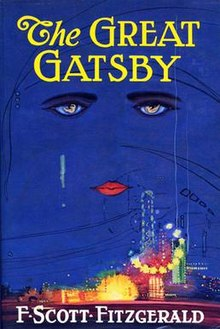
\includegraphics[width=0.25\textwidth]{images/jacket.jpg}
   \caption{The Great Gatsby}
\end{figure}

In my younger and more vulnerable years my father gave me some advice that I've been turning over in my mind ever since.

"Whenever you feel like criticising any one," he told me, "just
remember that all the people in this world haven't had the advantages
that you've had."

He didn't say any more but we've always been unusually communicative
in a reserved way, and I understood that he meant a great deal more
than that. In consequence I'm inclined to reserve all judgements,
a habit that has opened up many curious natures to me and also
made me the victim of not a few veteran bores. The abnormal mind
is quick to detect and attach itself to this quality when it
appears in a normal person, and so it came about that in college I
was unjustly accused of being a politician, because I was privy to the
secret griefs of wild, unknown men. Most of the confidences were
unsought--frequently I have feigned sleep, preoccupation, or a hostile
levity when I realised by some unmistakable sign that an intimate
revelation was quivering on the horizon--for the intimate revelations
of young men or at least the terms in which they express them are
usually plagiarist and marred by obvious suppression. Reserving
judgements is a matter of infinite hope. I am still a little afraid of
missing something if I forget that, as my father snobbishly suggested,
and I snobbishly repeat, a sense of the fundamental decencies is
parcelled out unequally at birth.

And, after boasting this way of my tolerance, I come to the admission
that it has a limit. Conduct may be founded on the hard rock or the wet
marshes but after a certain point I don't care what it's founded on.
When I came back from the East last autumn I felt that I wanted the
world to be in uniform and at a sort of moral attention forever; I
wanted no more riotous excursions with privileged glimpses into the
human heart. Only Gatsby, the man who gives his name to this book, was
exempt from my reaction--Gatsby who represented everything for which I
have an unaffected scorn. If personality is an unbroken series of
successful gestures, then there was something gorgeous about him, some
heightened sensitivity to the promises of life, as if he were related
to one of those intricate machines that register earthquakes ten
thousand miles away. This responsiveness had nothing to do with that
flabby impressionability which is dignified under the name of the
"creative temperament"--it was an extraordinary gift for hope, a romantic
readiness such as I have never found in any other person and which it
is not likely I shall ever find again. No--Gatsby turned out all right
at the end; it is what preyed on Gatsby, what foul dust floated in the
wake of his dreams that temporarily closed out my interest in the
abortive sorrows and short-winded elation of men.


My family have been prominent, well-to-do people in this middle-western
city for three generations. The Carraways are something of a clan and we
have a tradition that we're descended from the Dukes of Buccleuch, but the
actual founder of my line was my grandfather's brother who came here in
fifty-one, sent a substitute to the Civil War and started the wholesale
hardware business that my father carries on today.

I never saw this great-uncle but I'm supposed to look like him--with
special reference to the rather hard-boiled painting that hangs in
Father's office. I graduated from New Haven in 1915, just a quarter of a
century after my father, and a little later I participated in that
delayed Teutonic migration known as the Great War. I enjoyed the
counter-raid so thoroughly that I came back restless. Instead of being
the warm centre of the world the middle-west now seemed like the
ragged edge of the universe--so I decided to go east and learn the bond
business. Everybody I knew was in the bond business so I supposed it
could support one more single man. All my aunts and uncles talked it
over as if they were choosing a prep-school for me and finally said,
"Why--ye-es" with very grave, hesitant faces. Father agreed to finance
me for a year and after various delays I came east, permanently, I
thought, in the spring of twenty-two.

The practical thing was to find rooms in the city but it was a warm
season and I had just left a country of wide lawns and friendly trees,
so when a young man at the office suggested that we take a house
together in a commuting town it sounded like a great idea. He found
the house, a weather beaten cardboard bungalow at eighty a month, but
at the last minute the firm ordered him to Washington and I went out
to the country alone. I had a dog, at least I had him for a few days
until he ran away, and an old Dodge and a Finnish woman who made my bed
and cooked breakfast and muttered Finnish wisdom to herself over the
electric stove.

It was lonely for a day or so until one morning some man, more recently
arrived than I, stopped me on the road.

"How do you get to West Egg village?" he asked helplessly.

I told him. And as I walked on I was lonely no longer. I was a guide, a
pathfinder, an original settler. He had casually conferred on me the
freedom of the neighbourhood.

And so with the sunshine and the great bursts of leaves growing on the
trees--just as things grow in fast movies--I had that familiar
conviction that life was beginning over again with the summer.

There was so much to read for one thing and so much fine health to be
pulled down out of the young breath-giving air. I bought a dozen
volumes on banking and credit and investment securities and they stood
on my shelf in red and gold like new money from the mint, promising to
unfold the shining secrets that only Midas and Morgan and Maecenas
knew. And I had the high intention of reading many other books besides.
I was rather literary in college--one year I wrote a series of very
solemn and obvious editorials for the "Yale News"--and now I was going
to bring back all such things into my life and become again that most
limited of all specialists, the "well-rounded man." This isn't just an
epigram--life is much more successfully looked at from a single window,
after all.

It was a matter of chance that I should have rented a house in one of
the strangest communities in North America. It was on that slender
riotous island which extends itself due east of New York and where
there are, among other natural curiosities, two unusual formations of
land. Twenty miles from the city a pair of enormous eggs, identical in
contour and separated only by a courtesy bay, jut out into the most
domesticated body of salt water in the Western Hemisphere, the great
wet barnyard of Long Island Sound. They are not perfect ovals--like the
egg in the Columbus story they are both crushed flat at the contact
end--but their physical resemblance must be a source of perpetual
confusion to the gulls that fly overhead. To the wingless a more
arresting phenomenon is their dissimilarity in every particular except
shape and size.

I lived at West Egg, the--well, the less fashionable of the two, though
this is a most superficial tag to express the bizarre and not a little
sinister contrast between them. My house was at the very tip of the
egg, only fifty yards from the Sound, and squeezed between two huge
places that rented for twelve or fifteen thousand a season. The one on
my right was a colossal affair by any standard--it was a factual
imitation of some Hôtel de Ville in Normandy, with a tower on one side,
spanking new under a thin beard of raw ivy, and a marble swimming pool
and more than forty acres of lawn and garden. It was Gatsby's mansion.
Or rather, as I didn't know Mr. Gatsby it was a mansion inhabited by
a gentleman of that name. My own house was an eye-sore, but it was a
small eye-sore, and it had been overlooked, so I had a view of the
water, a partial view of my neighbour's lawn, and the consoling
proximity of millionaires--all for eighty dollars a month.

Across the courtesy bay the white palaces of fashionable East Egg
glittered along the water, and the history of the summer really begins
on the evening I drove over there to have dinner with the Tom
Buchanans. Daisy was my second cousin once removed and I'd known Tom
in college. And just after the war I spent two days with them in
Chicago.

Her husband, among various physical accomplishments, had been one of
the most powerful ends that ever played football at New Haven--a
national figure in a way, one of those men who reach such an acute
limited excellence at twenty-one that everything afterward savours of
anti-climax. His family were enormously wealthy--even in college his
freedom with money was a matter for reproach--but now he'd left Chicago
and come east in a fashion that rather took your breath away: for
instance he'd brought down a string of polo ponies from Lake Forest.
It was hard to realise that a man in my own generation was wealthy
enough to do that.

Why they came east I don't know. They had spent a year in France, for no
particular reason, and then drifted here and there unrestfully wherever
people played polo and were rich together. This was a permanent move,
said Daisy over the telephone, but I didn't believe it--I had no sight
into Daisy's heart but I felt that Tom would drift on forever seeking
a little wistfully for the dramatic turbulence of some irrecoverable
football game.

And so it happened that on a warm windy evening I drove over to East
Egg to see two old friends whom I scarcely knew at all. Their house was
even more elaborate than I expected, a cheerful red and white Georgian
Colonial mansion overlooking the bay. The lawn started at the beach
and ran toward the front door for a quarter of a mile, jumping over
sun-dials and brick walks and burning gardens--finally when it reached
the house drifting up the side in bright vines as though from the
momentum of its run. The front was broken by a line of French windows,
glowing now with reflected gold, and wide open to the warm windy
afternoon, and Tom Buchanan in riding clothes was standing with his
legs apart on the front porch.
% $$ SQNR_{p} = (6.02N) + 1.76 + ((20L) +10)log_{10}(OSR) - 10log_{10}(\frac{\pi^{2L}}{(2*L)+1})$$


\end{document}
